% Created by tikzDevice version 0.12
% !TEX encoding = UTF-8 Unicode
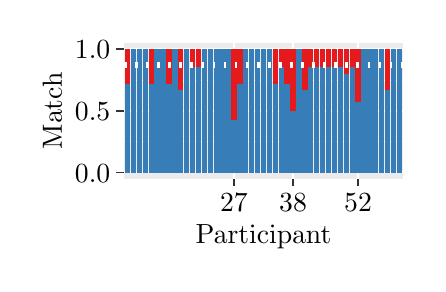
\begin{tikzpicture}[x=1pt,y=1pt]
\definecolor{fillColor}{RGB}{255,255,255}
\path[use as bounding box,fill=fillColor,fill opacity=0.00] (0,0) rectangle (141.12, 85.43);
\begin{scope}
\path[clip] (  0.00,  0.00) rectangle (141.12, 85.43);
\definecolor{drawColor}{RGB}{255,255,255}
\definecolor{fillColor}{RGB}{255,255,255}

\path[draw=drawColor,line width= 0.6pt,line join=round,line cap=round,fill=fillColor] ( -0.00,  0.00) rectangle (141.12, 85.43);
\end{scope}
\begin{scope}
\path[clip] ( 34.81, 30.86) rectangle (135.62, 79.93);
\definecolor{fillColor}{gray}{0.92}

\path[fill=fillColor] ( 34.81, 30.86) rectangle (135.62, 79.93);
\definecolor{drawColor}{RGB}{255,255,255}

\path[draw=drawColor,line width= 0.3pt,line join=round] ( 34.81, 44.25) --
	(135.62, 44.25);

\path[draw=drawColor,line width= 0.3pt,line join=round] ( 34.81, 66.55) --
	(135.62, 66.55);

\path[draw=drawColor,line width= 0.6pt,line join=round] ( 34.81, 33.09) --
	(135.62, 33.09);

\path[draw=drawColor,line width= 0.6pt,line join=round] ( 34.81, 55.40) --
	(135.62, 55.40);

\path[draw=drawColor,line width= 0.6pt,line join=round] ( 34.81, 77.70) --
	(135.62, 77.70);

\path[draw=drawColor,line width= 0.6pt,line join=round] ( 74.53, 30.86) --
	( 74.53, 79.93);

\path[draw=drawColor,line width= 0.6pt,line join=round] ( 95.89, 30.86) --
	( 95.89, 79.93);

\path[draw=drawColor,line width= 0.6pt,line join=round] (119.39, 30.86) --
	(119.39, 79.93);
\definecolor{fillColor}{RGB}{55,126,184}

\path[fill=fillColor] ( 35.13, 33.09) rectangle ( 37.05, 64.96);
\definecolor{fillColor}{RGB}{228,26,28}

\path[fill=fillColor] ( 35.13, 64.96) rectangle ( 37.05, 77.70);
\definecolor{fillColor}{RGB}{55,126,184}

\path[fill=fillColor] ( 37.26, 33.09) rectangle ( 39.18, 77.70);

\path[fill=fillColor] ( 39.40, 33.09) rectangle ( 41.32, 77.70);

\path[fill=fillColor] ( 41.53, 33.09) rectangle ( 43.46, 77.70);

\path[fill=fillColor] ( 43.67, 33.09) rectangle ( 45.59, 64.96);
\definecolor{fillColor}{RGB}{228,26,28}

\path[fill=fillColor] ( 43.67, 64.96) rectangle ( 45.59, 77.70);
\definecolor{fillColor}{RGB}{55,126,184}

\path[fill=fillColor] ( 45.81, 33.09) rectangle ( 47.73, 77.70);

\path[fill=fillColor] ( 47.94, 33.09) rectangle ( 49.86, 77.70);

\path[fill=fillColor] ( 50.08, 33.09) rectangle ( 52.00, 64.96);
\definecolor{fillColor}{RGB}{228,26,28}

\path[fill=fillColor] ( 50.08, 64.96) rectangle ( 52.00, 77.70);
\definecolor{fillColor}{RGB}{55,126,184}

\path[fill=fillColor] ( 52.21, 33.09) rectangle ( 54.14, 77.70);

\path[fill=fillColor] ( 54.35, 33.09) rectangle ( 56.27, 62.83);
\definecolor{fillColor}{RGB}{228,26,28}

\path[fill=fillColor] ( 54.35, 62.83) rectangle ( 56.27, 77.70);
\definecolor{fillColor}{RGB}{55,126,184}

\path[fill=fillColor] ( 56.49, 33.09) rectangle ( 58.41, 77.70);

\path[fill=fillColor] ( 58.62, 33.09) rectangle ( 60.54, 71.33);
\definecolor{fillColor}{RGB}{228,26,28}

\path[fill=fillColor] ( 58.62, 71.33) rectangle ( 60.54, 77.70);
\definecolor{fillColor}{RGB}{55,126,184}

\path[fill=fillColor] ( 60.76, 33.09) rectangle ( 62.68, 71.33);
\definecolor{fillColor}{RGB}{228,26,28}

\path[fill=fillColor] ( 60.76, 71.33) rectangle ( 62.68, 77.70);
\definecolor{fillColor}{RGB}{55,126,184}

\path[fill=fillColor] ( 62.89, 33.09) rectangle ( 64.82, 77.70);

\path[fill=fillColor] ( 65.03, 33.09) rectangle ( 66.95, 77.70);

\path[fill=fillColor] ( 67.16, 33.09) rectangle ( 69.09, 77.70);

\path[fill=fillColor] ( 69.30, 33.09) rectangle ( 71.22, 77.70);

\path[fill=fillColor] ( 71.44, 33.09) rectangle ( 73.36, 77.70);

\path[fill=fillColor] ( 73.57, 33.09) rectangle ( 75.49, 52.21);
\definecolor{fillColor}{RGB}{228,26,28}

\path[fill=fillColor] ( 73.57, 52.21) rectangle ( 75.49, 77.70);
\definecolor{fillColor}{RGB}{55,126,184}

\path[fill=fillColor] ( 75.71, 33.09) rectangle ( 77.63, 64.96);
\definecolor{fillColor}{RGB}{228,26,28}

\path[fill=fillColor] ( 75.71, 64.96) rectangle ( 77.63, 77.70);
\definecolor{fillColor}{RGB}{55,126,184}

\path[fill=fillColor] ( 77.84, 33.09) rectangle ( 79.77, 77.70);

\path[fill=fillColor] ( 79.98, 33.09) rectangle ( 81.90, 77.70);

\path[fill=fillColor] ( 82.12, 33.09) rectangle ( 84.04, 77.70);

\path[fill=fillColor] ( 84.25, 33.09) rectangle ( 86.17, 77.70);

\path[fill=fillColor] ( 86.39, 33.09) rectangle ( 88.31, 77.70);

\path[fill=fillColor] ( 88.52, 33.09) rectangle ( 90.45, 64.96);
\definecolor{fillColor}{RGB}{228,26,28}

\path[fill=fillColor] ( 88.52, 64.96) rectangle ( 90.45, 77.70);
\definecolor{fillColor}{RGB}{55,126,184}

\path[fill=fillColor] ( 90.66, 33.09) rectangle ( 92.58, 71.33);
\definecolor{fillColor}{RGB}{228,26,28}

\path[fill=fillColor] ( 90.66, 71.33) rectangle ( 92.58, 77.70);
\definecolor{fillColor}{RGB}{55,126,184}

\path[fill=fillColor] ( 92.80, 33.09) rectangle ( 94.72, 64.96);
\definecolor{fillColor}{RGB}{228,26,28}

\path[fill=fillColor] ( 92.80, 64.96) rectangle ( 94.72, 77.70);
\definecolor{fillColor}{RGB}{55,126,184}

\path[fill=fillColor] ( 94.93, 33.09) rectangle ( 96.85, 55.40);
\definecolor{fillColor}{RGB}{228,26,28}

\path[fill=fillColor] ( 94.93, 55.40) rectangle ( 96.85, 77.70);
\definecolor{fillColor}{RGB}{55,126,184}

\path[fill=fillColor] ( 97.07, 33.09) rectangle ( 98.99, 77.70);

\path[fill=fillColor] ( 99.20, 33.09) rectangle (101.13, 62.83);
\definecolor{fillColor}{RGB}{228,26,28}

\path[fill=fillColor] ( 99.20, 62.83) rectangle (101.13, 77.70);
\definecolor{fillColor}{RGB}{55,126,184}

\path[fill=fillColor] (101.34, 33.09) rectangle (103.26, 71.33);
\definecolor{fillColor}{RGB}{228,26,28}

\path[fill=fillColor] (101.34, 71.33) rectangle (103.26, 77.70);
\definecolor{fillColor}{RGB}{55,126,184}

\path[fill=fillColor] (103.47, 33.09) rectangle (105.40, 71.33);
\definecolor{fillColor}{RGB}{228,26,28}

\path[fill=fillColor] (103.47, 71.33) rectangle (105.40, 77.70);
\definecolor{fillColor}{RGB}{55,126,184}

\path[fill=fillColor] (105.61, 33.09) rectangle (107.53, 71.33);
\definecolor{fillColor}{RGB}{228,26,28}

\path[fill=fillColor] (105.61, 71.33) rectangle (107.53, 77.70);
\definecolor{fillColor}{RGB}{55,126,184}

\path[fill=fillColor] (107.75, 33.09) rectangle (109.67, 71.33);
\definecolor{fillColor}{RGB}{228,26,28}

\path[fill=fillColor] (107.75, 71.33) rectangle (109.67, 77.70);
\definecolor{fillColor}{RGB}{55,126,184}

\path[fill=fillColor] (109.88, 33.09) rectangle (111.80, 71.33);
\definecolor{fillColor}{RGB}{228,26,28}

\path[fill=fillColor] (109.88, 71.33) rectangle (111.80, 77.70);
\definecolor{fillColor}{RGB}{55,126,184}

\path[fill=fillColor] (112.02, 33.09) rectangle (113.94, 71.33);
\definecolor{fillColor}{RGB}{228,26,28}

\path[fill=fillColor] (112.02, 71.33) rectangle (113.94, 77.70);
\definecolor{fillColor}{RGB}{55,126,184}

\path[fill=fillColor] (114.15, 33.09) rectangle (116.08, 68.78);
\definecolor{fillColor}{RGB}{228,26,28}

\path[fill=fillColor] (114.15, 68.78) rectangle (116.08, 77.70);
\definecolor{fillColor}{RGB}{55,126,184}

\path[fill=fillColor] (116.29, 33.09) rectangle (118.21, 71.33);
\definecolor{fillColor}{RGB}{228,26,28}

\path[fill=fillColor] (116.29, 71.33) rectangle (118.21, 77.70);
\definecolor{fillColor}{RGB}{55,126,184}

\path[fill=fillColor] (118.43, 33.09) rectangle (120.35, 58.58);
\definecolor{fillColor}{RGB}{228,26,28}

\path[fill=fillColor] (118.43, 58.58) rectangle (120.35, 77.70);
\definecolor{fillColor}{RGB}{55,126,184}

\path[fill=fillColor] (120.56, 33.09) rectangle (122.48, 77.70);

\path[fill=fillColor] (122.70, 33.09) rectangle (124.62, 77.70);

\path[fill=fillColor] (124.83, 33.09) rectangle (126.76, 77.70);

\path[fill=fillColor] (126.97, 33.09) rectangle (128.89, 77.70);

\path[fill=fillColor] (129.11, 33.09) rectangle (131.03, 62.83);
\definecolor{fillColor}{RGB}{228,26,28}

\path[fill=fillColor] (129.11, 62.83) rectangle (131.03, 77.70);
\definecolor{fillColor}{RGB}{55,126,184}

\path[fill=fillColor] (131.24, 33.09) rectangle (133.16, 77.70);

\path[fill=fillColor] (133.38, 33.09) rectangle (135.30, 77.70);

\path[draw=drawColor,line width= 2.3pt,dash pattern=on 1pt off 3pt ,line join=round] ( 34.81, 72.03) -- (135.62, 72.03);
\end{scope}
\begin{scope}
\path[clip] (  0.00,  0.00) rectangle (141.12, 85.43);
\definecolor{drawColor}{RGB}{0,0,0}

\node[text=drawColor,anchor=base east,inner sep=0pt, outer sep=0pt, scale=  1.00] at ( 29.86, 29.65) {0.0};

\node[text=drawColor,anchor=base east,inner sep=0pt, outer sep=0pt, scale=  1.00] at ( 29.86, 51.95) {0.5};

\node[text=drawColor,anchor=base east,inner sep=0pt, outer sep=0pt, scale=  1.00] at ( 29.86, 74.26) {1.0};
\end{scope}
\begin{scope}
\path[clip] (  0.00,  0.00) rectangle (141.12, 85.43);
\definecolor{drawColor}{gray}{0.20}

\path[draw=drawColor,line width= 0.6pt,line join=round] ( 32.06, 33.09) --
	( 34.81, 33.09);

\path[draw=drawColor,line width= 0.6pt,line join=round] ( 32.06, 55.40) --
	( 34.81, 55.40);

\path[draw=drawColor,line width= 0.6pt,line join=round] ( 32.06, 77.70) --
	( 34.81, 77.70);
\end{scope}
\begin{scope}
\path[clip] (  0.00,  0.00) rectangle (141.12, 85.43);
\definecolor{drawColor}{gray}{0.20}

\path[draw=drawColor,line width= 0.6pt,line join=round] ( 74.53, 28.11) --
	( 74.53, 30.86);

\path[draw=drawColor,line width= 0.6pt,line join=round] ( 95.89, 28.11) --
	( 95.89, 30.86);

\path[draw=drawColor,line width= 0.6pt,line join=round] (119.39, 28.11) --
	(119.39, 30.86);
\end{scope}
\begin{scope}
\path[clip] (  0.00,  0.00) rectangle (141.12, 85.43);
\definecolor{drawColor}{RGB}{0,0,0}

\node[text=drawColor,anchor=base,inner sep=0pt, outer sep=0pt, scale=  1.00] at ( 74.53, 19.03) {27};

\node[text=drawColor,anchor=base,inner sep=0pt, outer sep=0pt, scale=  1.00] at ( 95.89, 19.03) {38};

\node[text=drawColor,anchor=base,inner sep=0pt, outer sep=0pt, scale=  1.00] at (119.39, 19.03) {52};
\end{scope}
\begin{scope}
\path[clip] (  0.00,  0.00) rectangle (141.12, 85.43);
\definecolor{drawColor}{RGB}{0,0,0}

\node[text=drawColor,anchor=base,inner sep=0pt, outer sep=0pt, scale=  1.00] at ( 85.21,  7.44) {Participant};
\end{scope}
\begin{scope}
\path[clip] (  0.00,  0.00) rectangle (141.12, 85.43);
\definecolor{drawColor}{RGB}{0,0,0}

\node[text=drawColor,rotate= 90.00,anchor=base,inner sep=0pt, outer sep=0pt, scale=  1.00] at ( 12.39, 55.40) {Match};
\end{scope}
\end{tikzpicture}
